\documentclass[10pt,twocolumn,letterpaper]{article}
%\usepackage[latin1]{inputenc}

%\usepackage{url}
%\usepackage{booktabs}

\usepackage{cvpr}
\usepackage{times}
\usepackage{epsfig}
\usepackage{graphicx}
\usepackage{amsmath}
\usepackage{amssymb}
\usepackage{amsmath}
\usepackage{amsfonts}
\usepackage{subfigure}
\usepackage{nonfloat}
\usepackage{url}
\usepackage{textcomp} % for textonehalf
%\usepackage{subref}
\graphicspath{{imgs/}}

\usepackage{xspace}
\renewcommand*{\eg}{e.g.\@\xspace}
\renewcommand*{\ie}{i.e.\@\xspace}
\newcommand*{\ea}{et al.\@\xspace}
%\renewcommand{\arraystretch}{1.5}

\cvprfinalcopy % *** Uncomment this line for the final submission

\def\cvprPaperID{****} % *** Enter the CVPR Paper ID here
\def\httilde{\mbox{\tt\raisebox{-.5ex}{\symbol{126}}}}

\newcommand{\prob}{Pr}
\newcommand{\imregion}{\mathcal{R}}
\newcommand{\occ}{o}
\newcommand{\basisshape}{B}
\newcommand{\pcloud}{\mathcal{P}}
\newcommand{\point}{\mathbf{p}}
\newcommand{\normal}{\mathbf{n}}
\newcommand{\ray}{\mathbf{R}}
\newcommand{\degree}{^{\circ}}
\newcommand{\rgbdimage}{\mathcal{D}}

\definecolor{red}{rgb}{0.95,0.4,0.4}
\definecolor{blue}{rgb}{0.4,0.4,0.95}
\definecolor{darkred}{rgb}{0.8,0,0}
\definecolor{darkgreen}{rgb}{0,0.5,0}
\definecolor{grey}{rgb}{0.6,0.6,0.6}

\newcommand{\todo}[1]{\textcolor{red}{TODO: #1}}
\newcommand{\note}[1]{\textcolor{blue}{NOTE: #1}}
\newcommand{\status}[1]{\textcolor{blue}{Status: #1}}
\newcommand{\add}[1]{\textcolor{darkgreen}{#1}}
\newcommand{\remove}[1]{\textcolor{grey}{#1}}



%[citecounter=true, style=ieee]
%\usepackage{biblatex}
%\addbibresource{bibtex/strings.bib}
%\addbibresource{bibtex/main.bib}
%\addbibresource{bibtex/crossrefs.bib}
%addbibresource{\jobname.bib}


\title{Predicting Voxel Occupancy From a Single RGBD Image}

%\author{Michael Firman, Gabriel Brostow, Simon Julier \ea}

\begin{document}


\maketitle

\begin{abstract}
	Gaining a representation of the geometry of a scene is an essential task for many applications including robotic navigation, scene re-lighting and object manipulation. 
	Most existing works to recover the scene geometry rely on combining multiple views of the scene captured from many different directions or use of \emph{a priori} information about the expected semantic make-up of the scene.

	We present a method to predict whether or not each voxel in a scene is occupied given just a single RGBD image.
	We argue that objects of dissimilar semantic classes often share similar shapes; this allows for a limited training dataset to model the shape of a wide range of objects and hence estimate the hidden geometry of arbitrary scenes.

	Our method comprises of three main components:
    1) For each pixel in an RGBD image, we compute local features together with a novel regional features and use these to predict the thickness of the object at that point, using a Random Forest trained on multiple CAD models.
    2) To extend occluded surfaces
    3) Finally we combine and regularise the thickness predictions and occluded surface continuations to form a full probablistic distribution of occupancy for each voxel in the scene.
\end{abstract}

% \begin{figure}
%   \centering 
%   \subfigure[Input depth image]{%
%       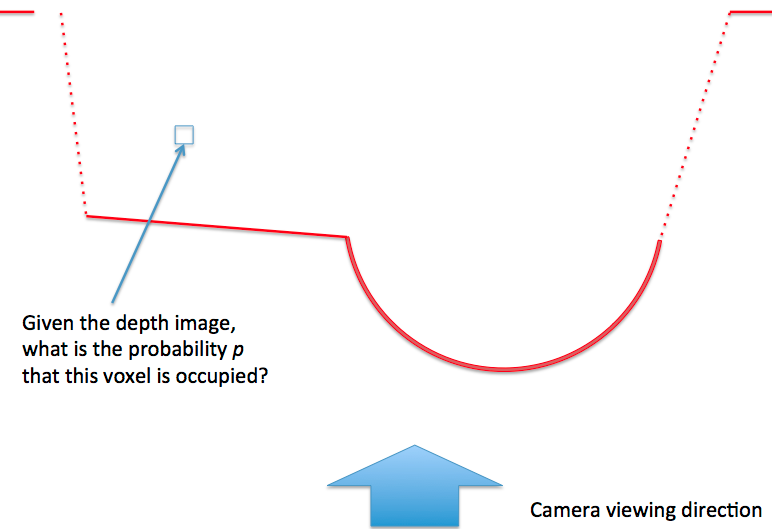
\includegraphics[width=0.8\columnwidth]{setup_ppt.png}}
%       \hfill
%   \subfigure[Ground truth output]{%
%       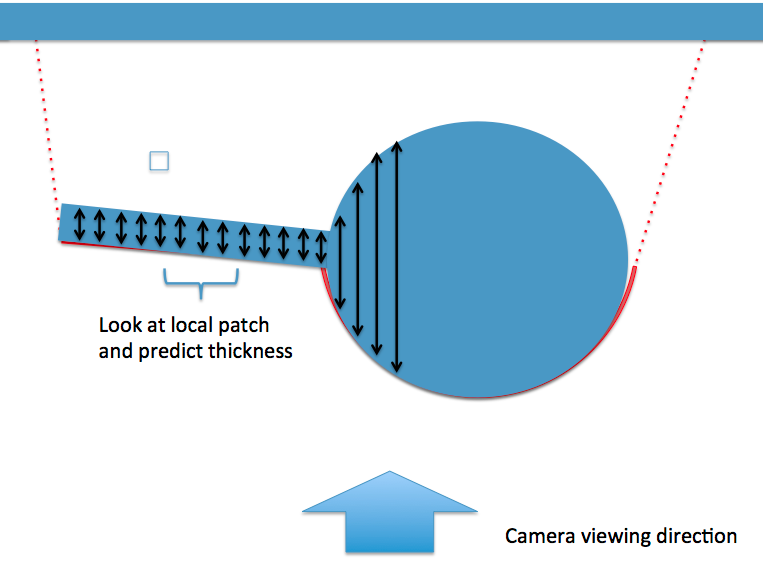
\includegraphics[width=0.8\columnwidth]{ground_truth_ppt.png}} \\
%   \caption{Given a depth image of a scene, \eg as depicted in 2D in (a), the aim is to predict the full, occupied volume of the scene (e.g. (b)).}
%   \label{fig:intro}
% \end{figure}

\section{Introduction}

% --- even with the use of depth sensors to capture data (\eg \cite{izadi-uist-2011}).
 % before these separate views are combined together.
For a robot to navigate through a cluttered room, an idea of which areas of 3D space are vacantis essential to avoid obstacles.
In order to acquire such a 3D occupancy model, however, a scene must be viewed from multiple angles.
This poses a chicken-and-egg problem: To capture the occupancy model the robot must navigate through the room, while the robot requires an occupancy model to navigate.

To solve this problem an initial estimate of the occupancy of each part of the scene can be made given an initial limited data set; as further observances are made this prior estimate can be overwritten by observed data.
This problem of estimating the unseen areas of the scene is ill-posed and can be very challenging; this is the problem we tackle in this paper.
%, it is possible to make sensible predictions about some areas.

If prior knowledge is available about the objects present in the scene in the form of 3D models, then these models can be fitted to the scene \cite{hinterstoisser-accv-2012, drost-3dimpvt-2012, rusu-iros-2010}, allowing the missing parts of the scene to be inferred.
This relies on having a detailed model of every item that could possibly be seen, which is infeasible for most practical situations.
Similarly, if the class can be inferred then a more generic class-level model can be fitted to a part of the scene \cite{cocias-cgvcv-2013, prisacariu-iccv-2011}; however, this relies on availability of such a class-level model, and the accuracy of an object classifier.
If we can accurately detect symmetry it is possible to make use of this to complete some types of objects (\eg \cite{law-cviu-2010, thrun-iccv-2005, kroemer-humanoids-2012}). 
However, using symmetry for object completion is brittle --- an incorrectly guessed symmetrical transform can lead to a catastrophic mis-estimate of geometry --- and symmetry is only visible in a subset of objects in our world.

%This allows the missing parts of objects to be reconstructed


%\note{Address semantics - head-on? Could argue from the start that while people attempt to use semantics to reconstruct shape, semantics can fail, can be ambiguous and rely on slow classification.}

In this paper we take a data-driven approach to estimating the missing geometry of a scene.
Unlike many papers which tackle this as a mesh completion problem \cite{schnabel-eurographics-2009, ju-cst-2009, maybsilberman-eccv-2014}, we directly tackle the problem by predicting voxel occupancy:
The input to our algorithm is a single depth image, while the output is an estimate of the occupancy of every voxel within the camera frustum.
Unlike previous work on voxel occupancy prediction \cite{kim-iccv-2013}, we do not require any semantic predictions, and our prediction of occupancy can be complex \note{Add more here...}.


\begin{figure}[!t]
  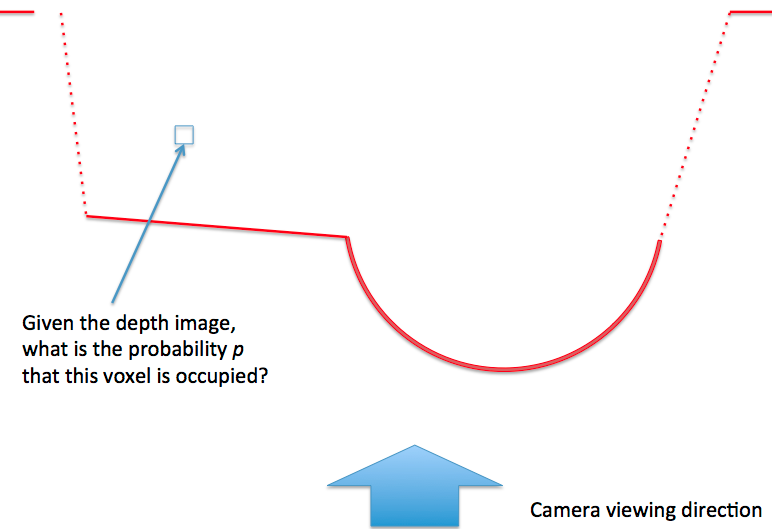
\includegraphics[width=0.98\columnwidth]{setup_ppt.png}
  \caption{Given a depth image of a scene, \eg as depicted in 2D in (a), the aim is to predict the full, occupied volume of the scene (e.g. (b)).}
  \label{fig:intro}
\end{figure}

%\subsection{Our algorithm}

%\paragraph{Occlusions}

We take inspiration from recent work which has segmented objects from images using silhouettes learned from different object classes \cite{kim-eccv-2012};
Their work showed that shape transcends class boundaries, enabling shape predictions to be made regardless of the accuracy of semantic classifiers.
Because we care about shape and voxel occupancy rather than semantic understanding, we are free to use training objects which differ in scale and semantic labelling from the objects being modelled in the scene.
This is key to our approach --- we are not reasoning about semantics of objects, but instead about object shape.

\paragraph{Aim of the system and overview}
Given a single RGBD image, our system predicts whether each voxel in the scene is occupied or not - in effect, we predict the voxelised occupancy grid of KinectFusion \cite{izadi-uist-2011}, but having been given only a single view of the scene instead of multiple views.

We achieve this by learning a mapping from local and novel semi-regional features to an object thickness, using a large collection of training objects and scenes.


%In effect we are hypothesising that any two rays that have a similar appearance from one angle are likely to share similarities in shape in the unobserved regions of the scene.

%In this respect we take inspiration from \cite{kim-eccv-2012}, where silhouettes from training objects are used to segment other objects from different classes.


%Occlusions and occlusion boundaries are a natural result of this projection from world space into image space.
%While often ignored or treated as a `nuicence', recently works have made explicit use of occlusion boundaries \cite{hoiem occlusion boundaires, segmenting simple objects}.

%Going from 2\textonehalf D to a full 3D representation is a challenging problem.
%Typically this has been approached by fusing together images from multiple viewpoints \cite{izadi-uist-2011}.

%Our world is naturally fully three-dimensional: We can think of every point in space as either being `occupied' by impenetrable solid matter, or as being `vacant', \ie transparent.
%A traditional camera image takes this 3D world and projects it onto a 2D plane.
%A great deal of information is lost in the process, as objects are flattened and occlusions prevent points behind those immediately visible to the camera ray from being observed. %, losing a whole dimension in the process.

%In recent years there have been great advances making affordable `3D' sensors available to capture a more complete representation of the world; these cameras, however, are still hampered by occlusions and technically only capture a 2\textonehalf D image.

%In many applications of depth cameras, however, it is not possible to gain a full view of all areas of the scene.

\paragraph{Other application areas}
It can be very useful for a computer system to know the geometry of hidden areas of a scene, for reasons such as:
\begin{itemize}
\item A wheeled robot entering a doorway of a cluttered room it has never seen before may wish to navigate to a target object at the far side. However, the floor surface may be occluded for much of the route, by furniture and other clutter.
\item If a single photo is captured from a mobile device with a depth camera attached, it could be useful to be able to relight the scene by digitally adding light sources. To cast realistic shadows, however, the full 3D geometry is required.
\item In multi-view reconstruction problems it can be good to have a prior over the shape of the scene from the first few frames, which can be replaced as more footage comes in. The prior can be used to solve the next-best-view problem, deciding where the camera should be moved to capture the most informative next image of the scene.
\end{itemize}

In these cases, we might wish to make an estimate of the geometry of the world, even if we have not seen the data to confirm the real 3D shape (figure \ref{fig:intro}).

%\begin{itemize}
%\item \textbf{Robotics} --- Helping a robot to plan a path around objects given only a single view of a scene, e.g. from a doorway. Also to help a robot plan grasping position on objects it can only see partial views of.
%\item \textbf{Scene relighting} --- Enabling realistic-looking shadows to be cast from a light moved to a new position in the image.
%\item \textbf{Object repositioning} --- Interactive repositioning of objects in the scene. Knowing the voxel occupancy allows a constraint to be placed on where objects can be moved to. (\eg Zheng \ea, Interactive images)
%\item \textbf{Multi-view reconstruction} --- An intial estimate for voxel occuapncy can be used as a prior during online multi-view reconstruction algorithms. This prior prediction would be overwritten with observed data as more footage is captured. The prior can help to solve the next-best-view problem.


\subsubsection{Contributions}
\begin{itemize}
\item A novel feature representation for a point which captures both local and region-level shape, while respecting occlusions.
\item A regularisation system for combining depth and surface predictions
\end{itemize}

% \begin{quote}
% Voxel occupancy is one approach for reconstructing the 3-dimensional shape of an object from multiple views. In voxel occupancy, the task is to produce a binary labeling of a set of voxels, that determines which voxels are filled and which are empty.
% \cite{snow-cvpr-2000}
% \end{quote}

\subsubsection{Problem statement}

\newcommand{\voxel}{\mathbf{v}}
%\newcommand{\occ}{f}

We assume the world to be made up of a regular 3D grid of voxels $V = \{\voxel_\gamma\}$, where $\voxel_\gamma = (i, j, k, \occ)$.
$(i, j, k)$  denotes the 3D position of the voxel in world space.
$\occ \in \{0, 1\}$ is a binary variable which takes the value $0$ if the voxel is vacant, and $1$ if it is occupied.

We treat a voxel as occupied if you cannot view its state from a camera moving around the scene from its start position.
So a voxel inside a closed cardboard box, while void of solid object, would be considered occupied.
On the other hand, a voxel on the inside of a cardboard box open at the top would be considered unoccupied.

Each scene is then captured in a single static depth image $\rgbdimage$ by a camera with extrinsics $H$ and intrinsics $K$. 
Assuming perspective projection, the location of each voxel projects into the camera to a position of:
\begin{equation}
[u, v, d]^T = K H [i, j, k]^T,
\end{equation}
where $(u,v)$ the position of the voxel in image coordinates, and $d$ is the  perpendicular distance from the camera centre to the voxel.
Finally, the value of each pixel $(u^*, v^*)$ in the depth image $\rgbdimage$ is given by the depth to the first occupied voxel along the camera ray:
\begin{equation}
\rgbdimage_{u^*,v^*} = \min_\gamma \left\{ d_{\gamma} : v_{\gamma} = 1, \lfloor u_{\gamma} \rfloor = u^*, \lfloor v_{\gamma} \rfloor = v^* \right\}.
\label{eqn:minimisation}
\end{equation}
%_{world \rightarrow camera} H_{grid \rightarrow world}

The $\min_d$ in (\ref{eqn:minimisation}) is the manifestation of occlusion: Each ray from the camera stops at the first occupied voxel it reaches.
The aim of our algorithm is to recover $V$ given $\rgbdimage$.


% %%%%%%%%%%%%%%%%%%%%%%%%%%%%%%%%%%%%%%%%%%%%%%%%%%%%%%%%%%%%%%%%%%%%%%%%%%%%%%%%
\section{Related work}
% %%%%%%%%%%%%%%%%%%%%%%%%%%%%%%%%%%%%%%%%%%%%%%%%%%%%%%%%%%%%%%%%%%%%%%%%%%%%%%%%

% \paragraph{Axes of variation of related works}
% Using local information (\eg smoothing) $\leftrightarrow$ using global information (\eg patching from other images)

%\note{Just some notes at the moment, organised into similar areas. Not much discussion yet.}
% Parametric models (Gaussian smoothing, CRFs) $\leftrightarrow$ non-parametric (patch-based)

% Care about semantic matching $\leftrightarrow$ Don't care about semantics

\note{
Previous works on completion can be categorised according to:
\begin{itemize}
\item their application domain, \ie mesh, 2D photo or voxel. 
\item whether they aim for aesthetic or absolute accuracy.
\item whether they take a data-driven approach or make use of heuristics.
\item if data used for completion come from within the same scene (\eg symmetry), from other scenes (\eg data-driven) or using heuristics.
\end{itemize}
I want to try to make use of these (or other) axes of variation in this section.
}

%%%%%%%%%%%%%%%%%%%%%%%%%%%%%%%%%%%%%%%%
\paragraph{Most similar in approach and aim to ours}
\cite{shen-tog-2012} use an assembly of parts from a CAD database to complete the unseen parts of a model given an RGBD image. 
While they demonstrate good results they assume they have semantic-specific models of the objects in the dataset.
Kim \ea \cite{kim-iccv-2013} use a CRF model over a voxel representation of a scene to simultaneously predict occupancy, visibility and semantical labelling of voxels from an RGBD image. 
For training, they use manually labelled top-down views of the scene. 
Their prediction of occupancy, however, is really just a Gaussian model. 
Their final labellings found from graph cuts over the CRF. 
They make the observation that the noisy observed values from a Kinect sensor cannot be relied upon and may need cleaning up.
%Silberman \ea \cite{silberman-eccv-2014} complete holes in partial KinectFusion meshes of indoor scenes.

%Fouhey \ea \cite{fouhey-iccv-2013} use the NYU dataset of RGBD images to learn how to predict the normal orientations for each pixel of an input RGB image. 
%In our case we are tackling a similar problem at a higher level --- we take RGBD as input, and aim to predict the full geometry of the scene.

\cite{guo-iccv-2013} use a single RGBD image to estimate the location and extent of the \emph{support surfaces} (\eg tabletops) in the scene. They do this by processing and analysing the geometry, before finally fitting shapes to the hypothesised support regions. They provide user-annotated 3D reconstructions of the full 3D space of the NYU dataset images, which could become useful for our work.

%%%%%%%%%%%%%%%%%%%%%%%%%%%%%%%%%%%%%%%%
\paragraph{Filling holes in meshes}
In the graphics community, there is a lot of work looking at the completion of missing and occluded parts of 3D meshes. 
For example, \cite{podolak-esgp-2005} fill holes in a mesh by enforcing watertightness across an octree structure, while \cite{schnabel-eurographics-2009} complete meshes by using primitives extracted from the areas of the scan without missing detail. 
A good overview of such mesh completion algorithms are given in \cite{ju-cst-2009}.

\cite{silberman-eccv-2014} complete meshes from partial KinFU reconstructions, \eg behind items of furniture.
They use this for augmeted realist situations, \eg allowing balls to bounce off floor in unseen areas.
They detect planes in the voxelised representation of the scene, and complete their contours in 2D using a novel CRF method.

Similar to mesh completion is super-resolution, \eg \cite{macaodha-eccv-2012}. 
This, like our problem, is ill-posed and relies on the repeatability and predictability of the world in order to find suitable matches.

%%%%%%%%%%%%%%%%%%%%%%%%%%%%%%%%%%%%%%%%
\paragraph{Image completion}
Image completion, such as \cite{hays-siggraph-2007, criminisi-cvpr-2003}, typically has the aim of getting a good visually plausible output irrespective of the accuracy compared to ground truth. 
The results can be very impressive.
Image completion typically uses region-based data-driven approaches, as it is very difficult to form generative models of image appearance.
For example, \cite{hays-siggraph-2007} look up possible completion regions in a large database of similar images, while \cite{criminisi-cvpr-2003} in-paint by selecting and combining multiple plausible patches from other regions of the input image.

%Depth images are a more complex beast than meshes and 2D images, and RGBD datasets on the order of millions of images do not yet exist, so we need to take a different approach.

%\paragraph{Super-resolution}
%A seminal paper in this field is \cite{freeman-ijcv-2000}, patches from generic training images are used in super-resolution for coarse-grained images. They use Bayesian belief propagation to find the maximum posterior probability over a Markov network defined over the image.
%\cite{chang-tor-2007} complete a robot's map of an environment using parts of the already observed world to  `patch in' missing areas of the current map.

%%%%%%%%%%%%%%%%%%%%%%%%%%%%%%%%%%%%%%%%
\paragraph{Symmetry}
Law and Aliaga \cite{law-cviu-2010} use symmetry to complete partial views. 
They are limited to only completing partial views; they rely on all objects being symmetrical; and they need user input.
Similarly, \cite{thrun-iccv-2005} and \cite{kroemer-humanoids-2012} use symmetry to complete models from a single depth view. 
They both demonstrate results on isolated objects, but not on more complex or cluttered scenes. 
The constraint of requiring axes of symmetry to both be present and accurately detected is a large limiting factor with these approaches.
also: \url{http://publik.tuwien.ac.at/files/PubDat_198335.pdf}

%%%%%%%%%%%%%%%%%%%%%%%%%%%%%%%%%%%%%%%%
\paragraph{3D from a single 2D image}
Reconstructing PASCAL VOC - \cite{vicente-cvpr-2014}

%%%%%%%%%%%%%%%%%%%%%%%%%%%%%%%%%%%%%%%%
\paragraph{Indoor room occupied space prediction}
\cite{hedau-cvpr-2012} seek to recover the free space in 2D images. They label ~500 images with box annotations, and aim to recover the bounding box layout of the scene in order to recover the free space.
\cite{bao-wacv-2014} use multiple images, before SfM and segmentation of the images. 
They then generate hypotheses of the layout. 
The hypotheses are chosen by evaluating their geometric cost, which is manually defined. 
%They cite a lot of papers which do scene reasoning from a single image, but they argue that the problem is ill-posed (which it is). 

Using a single image, many people fit bounding boxes and try to estimate the layout using high-level info about gravity, typical scene arrangements etc. 
For example \cite{choi-cvpr-2013, shao-siggraphasia-2014}.
The high-level reasoning gives a great opportunity to gain a quality scene reconstruction.
The problem with these methods is that they gives incredibly coarse occupation information; only a small subset of objects have a nice cuboid shape.
In addition, these methods do not degrade gracefully.
A small error in cuboid fitting can lead to a very large misclassification of volume.

\cite{lee-nips-2010} are another paper using a single image to estimate the layout of a room. 
Similarly, \cite{zhang-iccv-2013} infer the clutter and layout and support and segmentation and labelling from an RGBD image (using the NYU dataset).

A big work in this area is that by \cite{gupta-cvpr-2011}, who estimate voxel occupation before fitting boxes.

Satkin \ea \cite{satkin-bmvc-2012} use 3D models to do scene understanding from a single image, and they demonstrate results on room scenes such as bedrooms and living rooms. 
A key interest for me is that they first propose hypotheses, before rendering them with OpenGL.
This then feeds into a hypothesis scorer which says if their ideas are any good. 
They form their proposals in an expensive way: they moving the cad model along the (x, y) scene axes, and render the model in every location, and in each of 4 rotation configurations!

\paragraph{6DOF object pose estimation}
Our work is closely related to the problem of estimating the 6DOF pose of a known database of objects in cluttered scenes, such as \cite{hinterstoisser-accv-2012, drost-3dimpvt-2012, rusu-iros-2010}. 
These work in many different ways; \cite{drost-3dimpvt-2012} aggregate pairwise features in a hash table to find the pose estimation --- they assume just one database model, which is assumed to be in the scene. \cite{rusu-iros-2010} first segment the scene, before looking up each segment in their training dataset.
All the methods nonetheless share the training step of rendering a 3D object from multiple angles.

All these methods so far assume that the item in the scene has the exact same geometry of the training instances.
\cite{cocias-cgvcv-2013} take an alternative approach, where they have a single primitive object for each class, which they fit to the scene and allow to deform to account for inter-class variation.
\cite{prisacariu-iccv-2011} present a more developed version of this idea, where the latent axes of variation of the shape of the object being fitted are allowed to deform during the pose estimation. 
These latent axes are found using Gaussian processes.
This adaptive fitting of generic primitives to the specific instances seen in an image has seen practical application in the graphics community, where it has been used for an impressive interactive photo-editing application \cite{kholgade-siggraph-2014}.

\cite{zhang-eccv-2014} do indoor 3D semantic bounding box prediction using a single 2D panoramic image. They make heavy use of context to drive their predictions.
In our work, by not restricting ourselves to trying to find semantic correspondences, we are able to model the shape of a far greater range of test scenes without making any assumptions about their semantic makeup.

Render CAD models from multiple directions, combine with sliding window detector: \cite{song-eccv-2014}.


\paragraph{General motivation}

 \cite{nan-acm-2012}.

Big issue with ground truth. Most papers don't have proper ground truth and therefore can only really do qualitative results, \eg \cite{all the papers...}.

\paragraph{To add to related work:}
\begin{itemize}
\item Teaching 3D Geometry to Deformable Part Models
\item Things which cited voxel CRF...
Also: Amodal volume completion: 3D visual completion

Class specific: Single and sparse view 3D reconstruction by learning shape priors


%http://scholar.google.co.uk/scholar?safe=off&espv=2&bav=on.2,or.r_cp.r_qf.&bvm=bv.75775273,d.ZWU,pv.xjs.s.en.CtdJ7drbKko.O&ion=1&biw=1164&bih=816&um=1&ie=UTF-8&lr=&cites=16286130882256685425
\end{itemize}

%%%%%%%%%%%%%%%%%%%%%%%%%%%%%%%%%%%%%%%%%%%%%%%%%%%%%%%%%%%%%%%%%%%%%%%%%%%
\subsection{Application areas}
\note{Just some notes and refs which could go here, in intro or no-where}

\paragraph{Scene relighting}
\cite{ikeda-acpr-2013} perform scene relighting from a single RGBD image, but cannot recover shadows cast by objects in the scene.
On the other hand, \cite{xiao-cvpr-2014} use the RGBD information to automatically \textit{remove} hard and soft shadows from a single image.

\paragraph{Robotics and path planning}
Voxels or 2D occupancy grids are often used in robotics for path planning, and for maintaining a map of the environment. 
These are typically deterministic approaches, \eg \cite{jetchev-icra-2010}. Sometimes a state model is used to model the states of voxels being occupied, unoccupied or unknown --- the voxel states are then updated as more information is gathered from sensors \cite{toussaint-techreport-2007}.

\cite{stentz-icra-1994} introduced D*, an algorithm similar to A* but for path planing in partially unknown environments. 
The world is in boxes, with arrows pointing to the direction which should be taken.
More recently, \cite{plagemann-iros-2008} used Gaussian processes to fill in missing data in terrain models of environments, effectively treating terrain mapping as a regression problem.




\begin{figure}
  \centering 
  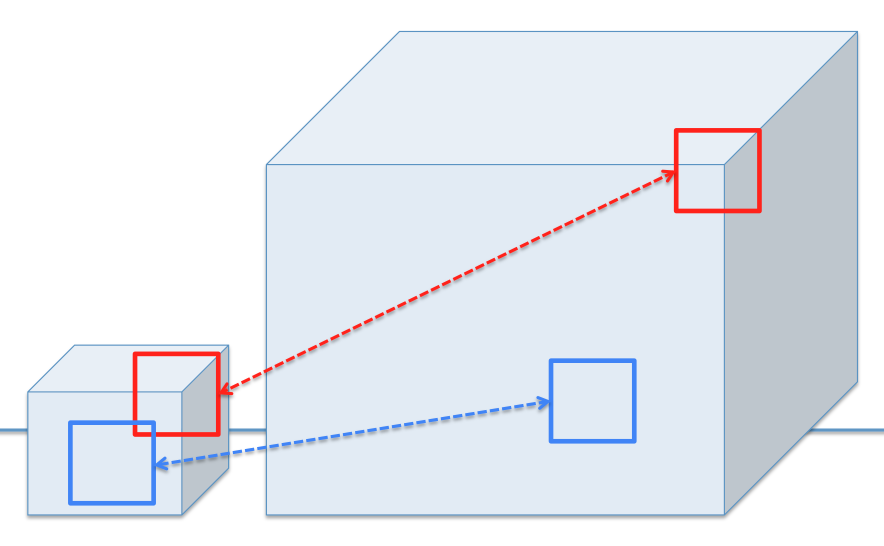
\includegraphics[width=0.9\columnwidth]{patch_sizes.png}
      
  \caption{Local, patch-type features do not give enough information to accurately predict depth. Here, two pairs of patches are marked. Each item in these pairs have identical local appearance. However, the thickness of the object at each patch location is very different. We use this to motivate the spider feature.}
\end{figure}


% %%%%%%%%%%%%%%%%%%%%%%%%%%%%%%%%%%%%%%%%%%%%%%%%%%%%%%%%%%%%%%%%%%%%%%%%%%%%%%%%
\section{Methodology}
% %%%%%%%%%%%%%%%%%%%%%%%%%%%%%%%%%%%%%%%%%%%%%%%%%%%%%%%%%%%%%%%%%%%%%%%%%%%%%%%%

Our approach is somewhat inspired by patch-based methods used for superresolution or similar of depth images. 

% Overview of the method --- Figure \ref{fig:pipeline}.


% General motivation for method. Do not want to rely on having exact matches in training set. 
% Instead, want to find a collection of good matches in the training set which, when combined, will give a sensible prediction of the voxel occupancy.
% We take a RANSAC-style approach to finding basis shapes: first we \emph{propose} a set of candidate shapes which roughly match the scene, before we next \emph{re-weight} these candidates according to how well they match the scene geometry. 

The aim of our thickness prediction function is to map a point $\point$ in the image to a scalar thickness $t$.


%%%%%%%%%%%%%%%%%%%%%%%%%%%%%%%%%%%%%%%%%%%%%%%%%%%%%%%%%%%%%%%%%%%%%%%%%%%%%%%%%
\subsection{Preprocessing and discontinuity mapping}
Describe here:
\begin{itemize}
\item Reprojecting the depth image into the colour camera
\item Smoothing - both citations
\item Types of edges (depth, colour, occluding etc)
\item Our method for depth edges
\item motivation - why do we care about occlusions?
\end{itemize}

We reason that discontinuities in depth images can be assigned a direction: one side of each edge is the occluder, the other is the occludee. 
We can compute the gradient of the depth edges using PCA on the edge pixels in image space.
We ensure that the final gradient at each edge pixel points in the direction of the occluded side.

We can then use the occlusion information in our feature computations --- see for example figure \ref{fig:occluded_region}.



\begin{figure}
    \centering 
    \subfigure[]{%
        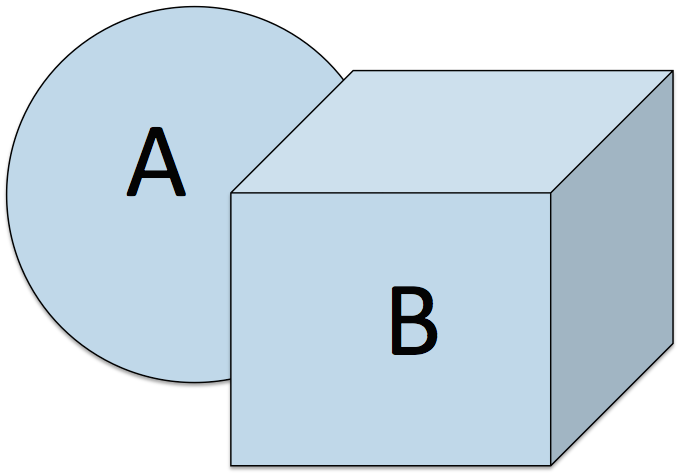
\includegraphics[width=0.45\columnwidth]{occlusion_a}}
        \hfill
    \subfigure[]{%
        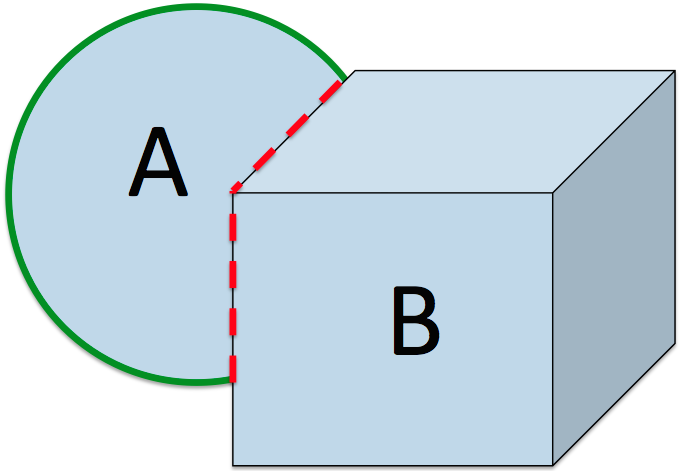
\includegraphics[width=0.45\columnwidth]{occlusion_b}} \\
    \caption{Where edges occur as a result of occlusion boundaries, the direction of the edge is important. The edge bounding region A can be divided into an \emph{occluding} portion (solid green) and an \emph{occluded} portion (dashed red).
    We can make a reasonable assumption that region A may extend behind object B past the occluded edge --- however, region A cannot continue sideways beyond its occluding edge.}
    \label{fig:occluded_region}
\end{figure}



%%%%%%%%%%%%%%%%%%%%%%%%%%%%%%%%%%%%%%%%%%%%%%%%%%%%%%%%%%%%%%%%%%%%%%%%%%%%%%%%%
\subsection{Features}
\note{Lots of papers \eg microsoft use local features in region of point. For thickness this doesn't cut the mustard, so we augment with region features. However, most region features ignore occlusions. We don't.}

Our method is to use local and regional featues extracted from the image around $\point$ to predict the thickness of the object at that point.
We use two novel features, which we describe in detail here. See also figure \ref{fig:features}.

\newcommand{\subwidth}{0.32\columnwidth}
\begin{figure*}
    \centering 
    \subfigure[Spider feature]{%
        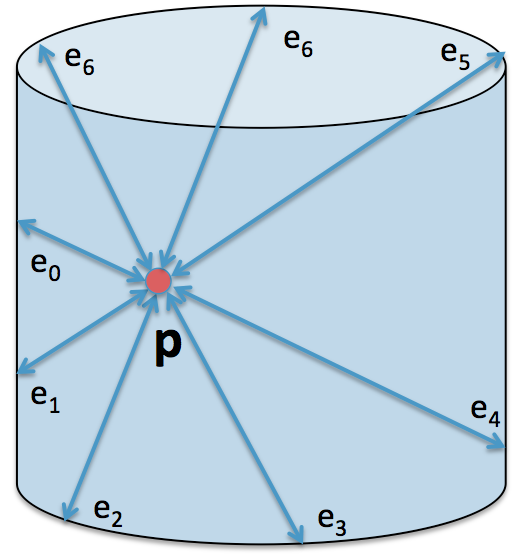
\includegraphics[width=\subwidth]{02_spider}}
        \hfill
    \subfigure[Occluded spider]{%
        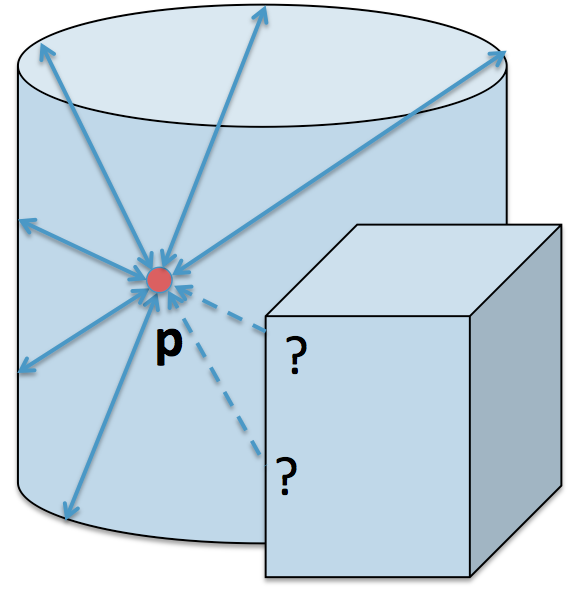
\includegraphics[width=\subwidth]{04_spider_occ}
        \label{fig:features:occluded_spider}}
        \hfill
    \subfigure[Cobweb feature]{%
        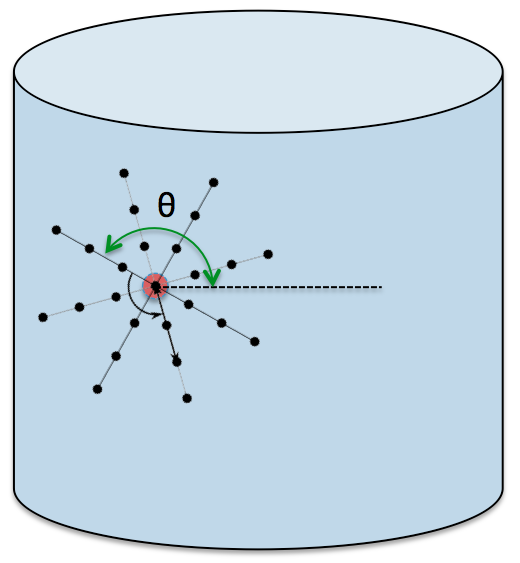
\includegraphics[width=\subwidth]{05_cobweb}}
        \hfill
    \caption{
    %(a) Each point on a depth image has an angle $\theta$ associated, which represents the direction of gradient of the depth. 
    (b) The spider features measure the distance between $\point$ and the edge points $e_{1, \cdots, 7}$.
    %(c) Because the spider features are computed relative to $\theta$, the resultant feature vector is invariant to object rotations in the camera plane.
    (d) Where the spider line emitted from $\point$ first hits an occluded edge, only a \textit{minimum} extent is known --- this case is denoted as \texttt{?} in this figure.
    (e) The cobweb feature measures the difference in depth between $\point$ and a set of points in the near vicinity of $\point$, arranged in a cobweb shape.}%
    \label{fig:features}
\end{figure*}



\begin{figure}
    \centering 
    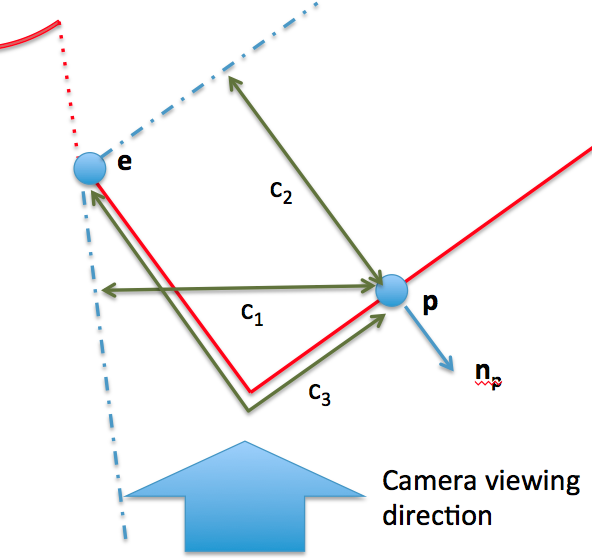
\includegraphics[width=1.0\columnwidth]{compass_features}
    \caption{We compute three flavours of compass features, which measure the distance between $\mathbb{p}$ and the edge point $\mathbb{e}$ in different ways. $c_1$ is the distance perpendicular to the camera direction; $c_2$ measures the depth of the object perpendicular to the normal at $\mathbb{p}$; while $c_3$ is the geodesic distance between $\mathbb{p}$ and $\mathbb{e}$.}
    \label{fig:compass_features}
\end{figure}


%It captures very similar data to a patch of the depth image; however, an image patch maintains a constant resolution across the selected region, while the cobweb feature becomes more coarse the farther from $\point$ it is.
%This property helps to reflect the 
\subsubsection{Cobweb feature}
The cobweb feature is a simple pairwise feature, inspired by \footnote{\url{http://research.microsoft.com/pubs/145347/bodypartrecognition.pdf}}, capturing the surface shape in the immediate vicinity of $\point$.
\begin{align}
f(i, j, \psi, t) &= \rgbdimage_{ij} - \rgbdimage_{ab} \\
a &= \left\lfloor i + \frac{tdf}{\rgbdimage_{ij}}  \sin(\psi) \right\rceil \\
b &= \left\lfloor j + \frac{tdf}{\rgbdimage_{ij}}  \cos(\psi) \right\rceil
\end{align}
where $f$ is the focal length of the camera and $d$ is a fixed constant in real-world coordinates. For our experiements we set $d=0.02m$ and we compute the cobweb feature for $\psi = [0\degree, 45\degree, \ldots, 315\degree]$, and $t = [1, 2, 3]$. 
The final cobweb feature is therefore 24-dimensional.
%Note also: ``If an offset pixel lies on the background or outside the bounds of the image, the depth probe dI (x0) is given a large positive constant value''.



\subsubsection{Spider features}
The spider feature captures the size and shape of the region in which $\point$ resides. 
Rather than explicitly computing region-level features, however, which may suffer from poor segmentations (and the problem with occlusion), we compute these features capturing the region's shape at the point level. 
We first compute an edge map for the image.
We again consider the set of angles $\phi$. Starting from $\point$, we cast a Bresenham line along the depth image until it hits an edge. 
We denote the point at which the edge was hit as $\point_{e}$.

For each line cast, we store
a) the geodesic distance between $\point$ and $\point_{e}$ along the depth surface, and 
b) the 3D distance between $\point$ and $\point_{e}$ along the direction of the normal at $\point$. (In practice, we take the point 95\% of the way between $\point$ and $\point_{e}$ in image space, as this helps to prevent problems with poor quality edge data).

The spider feature is therefore 16-dimensional.

While it captures a wide range of information about the region within which a point resides, the spider feature is extremely efficient to compute.
This is mainly due to the additive nature of the feature: The spider feature in direction $0\degree$ at $(i, j)$ can be computed from summing a small fraction 
We can compute the 16D spider feature for every point in a $640\times480$ image in less than 0.01s using unoptomised C++ code; we would expect a significant speedup were this to be implemented on a GPU.

\subsubsection{Occluded spider features}

We explicitly handle occlusion in the spider features. Where the spider feature first hits an occluded edge rather than an occluding edge, the true size of the object in that dimension is unknown (see figure \ref{fig:features:occluded_spider}).
However, we do have a \textit{minimum} size in that direction.
We use a generative model to sample the missing feature from the minimum size in that direction and the dimensions in all the other directions.

%We explicitly encode this unknown value --- in practice with \texttt{NaN} --- and the Random Forest can then make a sensible decision about what to do with it.

% \begin{figure}
%     \centering% 
%     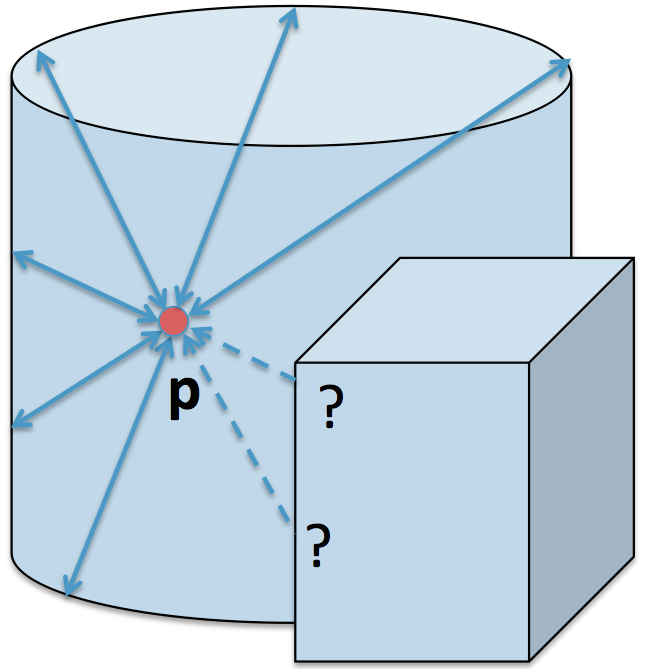
\includegraphics[width=0.7\columnwidth]{occlusion_spider.png}% 
%     \figcaption{The spider feature extends lines from $\point$ to the first occluding edge found along the path. Internal edges (e.g. those found in RGB space) are ignored. Where the line first hits an occluded edge, the true extent is unknown --- this case is denoted as \texttt{?} in this figure.}% 
%     \label{fig:occluded_spider}% 
% \end{figure}




%\subsubsection{}

%%%%%%%%%%%%%%%%%%%%%%%%%%%%%%%%%%%%%%%%%%%%%%%%%%%%%%%%%%%%%%%%%%%%%%%%%%%%%%%%%
\subsection{Thickness Forest}

We train a Random Forest using a total of 1,000,000 training examples extracted from 1,600 CAD models, each rendered from 42 different angles.


\subsection{Combining predictions}

\begin{figure}
    \centering% 
    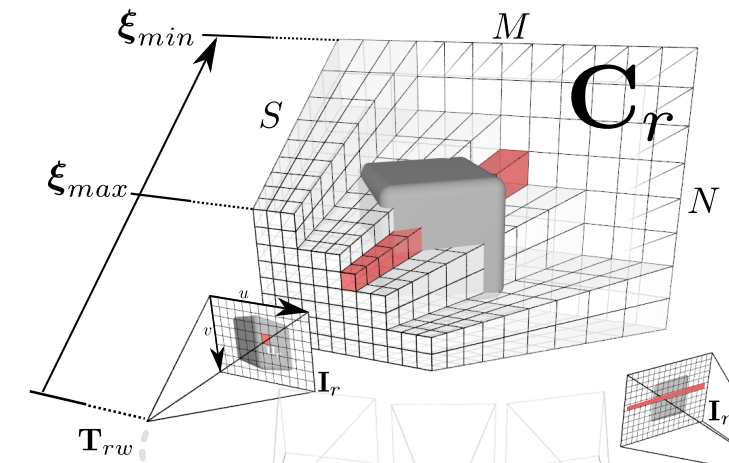
\includegraphics[width=1.0\columnwidth]{dtam_voxels.png}% 
    \figcaption{The warped voxelisation we make of our scene.
    The voxel space is a frustum grid, and each voxel is therefore a prismoidal hexahedron.
    Image from \cite{newcombe-iccv-2011} --- I should probably make a similar one.}% 
    \label{fig:dtam_voxels}% 
\end{figure}



%%%%%%%%%%%%%%%%%%%%%%%%%%%%%%%%%%%%%%%%%%%%%%%%%%%%%%%%%%%%%%%%%%%%%%%%%%%%%%%%
\section{Datasets used}
%%%%%%%%%%%%%%%%%%%%%%%%%%%%%%%%%%%%%%%%%%%%%%%%%%%%%%%%%%%%%%%%%%%%%%%%%%%%%%%%


%%%%%%%%%%%%%%%%%%%%%%%%%%%%%%%%%%%%%%%%%%%%%%%%%%%%%%%%%%%%%%%%%%%%%%%%%%%%%%%%
\section{Experiments}
%%%%%%%%%%%%%%%%%%%%%%%%%%%%%%%%%%%%%%%%%%%%%%%%%%%%%%%%%%%%%%%%%%%%%%%%%%%%%%%%


\begin{figure}
    \centering% 
    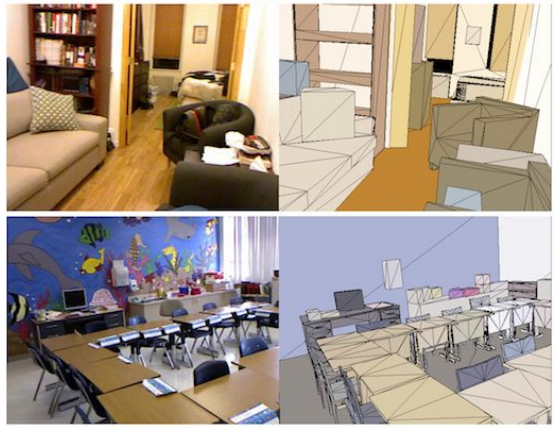
\includegraphics[width=1.0\columnwidth]{guo.png}% 
    \figcaption{Representation of objects in the NYU dataset, provided from \cite{guo-iccv-2013}.
    Not a perfect representation but perhaps reasonable to some extents.}% 
    \label{fig:guo_labels}% 
\end{figure}



\subsection{Database of CAD models}
Use the database from Fisher \ea \cite{fisher-siggraphasia-2012}.
1600 CAD models, each depth-rendered from 42 viewing angles using OpenGL.

\subsubsection{Potential test datasets}
\begin{itemize}
\item Create our own KinFu dataset
\item Kaparthy \ea --- would probably have to re-render their meshes.
Also don't have the TSDF etc. Lots of problems
\item NYU dataset --- classic dataset. Potential ground truth labels from \cite{guo-iccv-2013} (figure \ref{fig:guo_labels}) or \cite{kim-iccv-2013}.
\item \cite{fisher-siggraphasia-2012}, use their synthetic scenes (great for a first pass!)
\end{itemize}

\begin{figure}
    \centering% 
    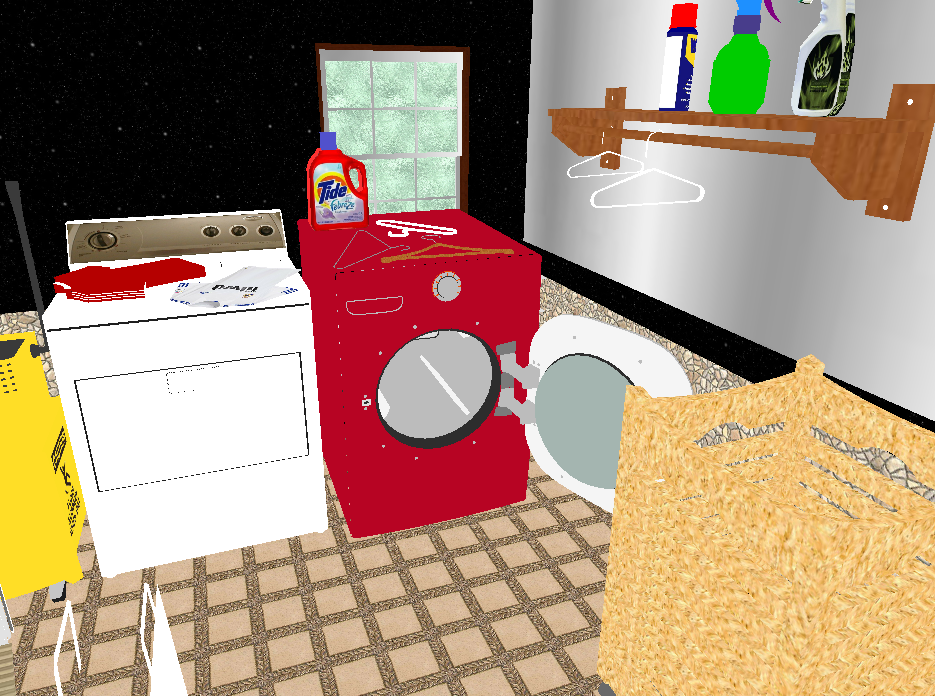
\includegraphics[width=1.0\columnwidth]{synth_scene.png}% 
    \figcaption{One of the user-created synthetic scenes from \cite{fisher-siggraphasia-2012}.}% 
    \label{fig:fisher_scene}% 
\end{figure}

% \section{Acknowledgements}
% Peter Gehler
% Oisin
% Malcolm
% Neill
% Prism group

{\small
%\bibliographystyle{plain}
\bibliographystyle{ieee}
\bibliography{bibtex/strings.bib,bibtex/main.bib,bibtex/crossrefs.bib}
}

%\printbibliography


\end{document}